\chapter{Port Security}\label{port-security}

\section{Intro to Port Security}\label{intro-to-port-security}

\begin{itemize}
\tightlist
\item
  PORT SECURITY is a security feature of Cisco SWITCHES
\item
  It allows you to control WHICH SOURCE MAC ADDRESS(ES) are allowed to
  enter the SWITCHPORT
\item
  If an unauthorized SOURCE MAC ADDRESS enters the PORT, an ACTION will
  be TAKEN

  \begin{itemize}
  \tightlist
  \item
    The DEFAULT action is to place the INTERFACE in an ``err-disabled''
    state
  \end{itemize}
\end{itemize}

\begin{figure}
\centering
\pandocbounded{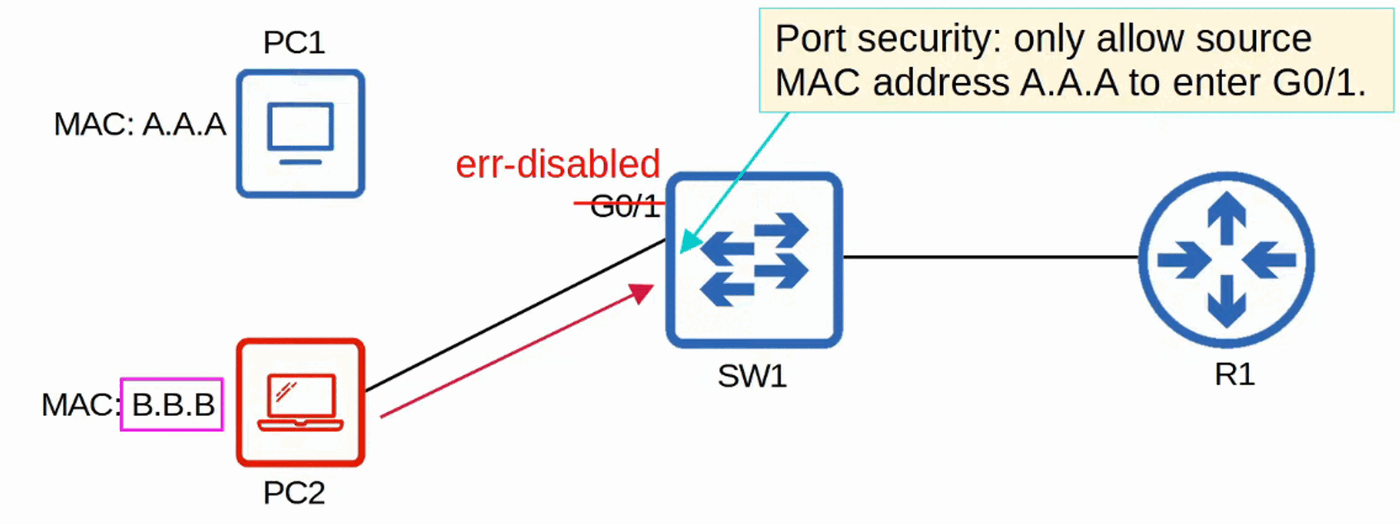
\includegraphics[keepaspectratio,alt={image}]{images/50-port-security/img-001.png}}
\end{figure}

\begin{itemize}
\tightlist
\item
  When you enable PORT SECURITY on an INTERFACE with the DEFAULT
  settings, one MAC ADDRESS is allowed

  \begin{itemize}
  \tightlist
  \item
    You can configure the ALLOWED MAC ADDRESS manually
  \item
    If you DO NOT configure it manually, the SWITCH will allow the first
    SOURCE MAC ADDRESS that enters the INTERFACE
  \end{itemize}
\item
  You can CHANGE the MAXIMUM number of MAC ADDRESSES allowed
\item
  A COMBINATION of manually configured MAC ADDRESSES and DYNAMICALLY
  LEARNED ADDRESSES is possible
\end{itemize}

\begin{figure}
\centering
\pandocbounded{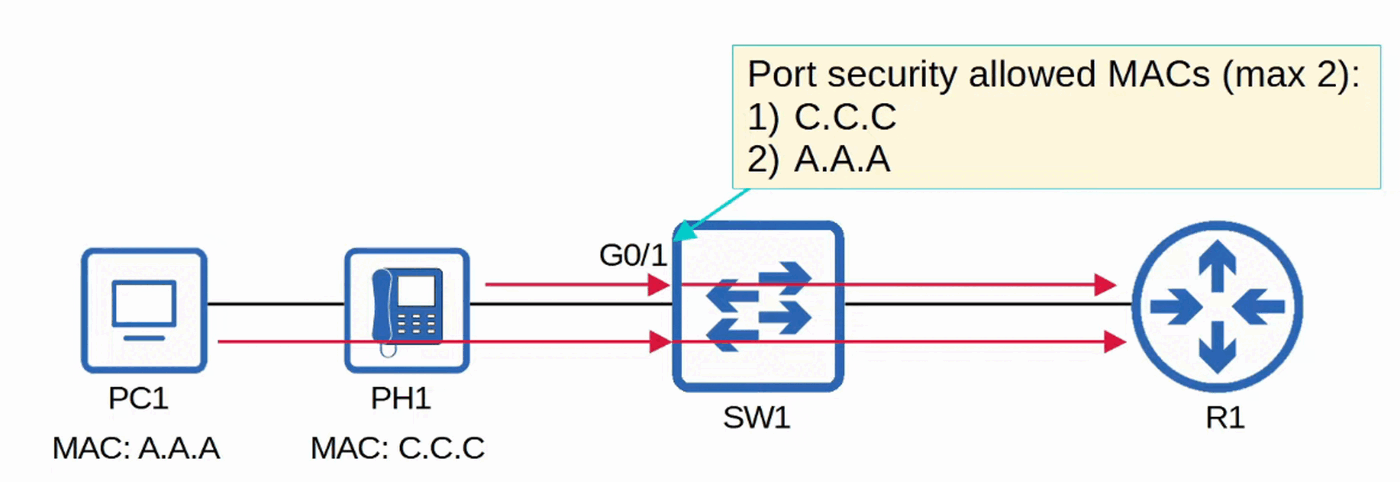
\includegraphics[keepaspectratio,alt={image}]{images/50-port-security/img-002.png}}
\end{figure}

WHY USE PORT SECURITY?

\begin{itemize}
\tightlist
\item
  PORT SECURITY allows NETWORK admins to control which DEVICES are
  allowed to access the NETWORK
\item
  However, MAC ADDRESS SPOOFING is a simple task

  \begin{itemize}
  \tightlist
  \item
    It is easy to configure a DEVICE to send FRAMES with a different
    SOURCE MAC ADDRESS
  \end{itemize}
\item
  Rather than manually specifying the MAC ADDRESSES allowed on each
  PORT, PORT SECURITY'S ability to limit the number of MAC ADDRESSES
  allowed on an INTERFACE is more useful
\item
  Think of the DHCP STARVATION ATTACK (DAY 48 LAB video)

  \begin{itemize}
  \tightlist
  \item
    The ATTACKER spoofed thousands of fake MAC ADDRESSES
  \item
    The DHCP SERVER assigned IP ADDRESSES to these fake MAC ADDRESSES,
    exhausting the DHCP POOL
  \item
    The SWITCH'S MAC ADDRESS table can also become full due to such an
    attack
  \end{itemize}
\item
  Limiting the NUMBER of MAC ADDRESSES on an INTERFACE can protect
  against those attacks
\end{itemize}

\section{Enabling Port Security}\label{enabling-port-security}

\begin{figure}
\centering
\pandocbounded{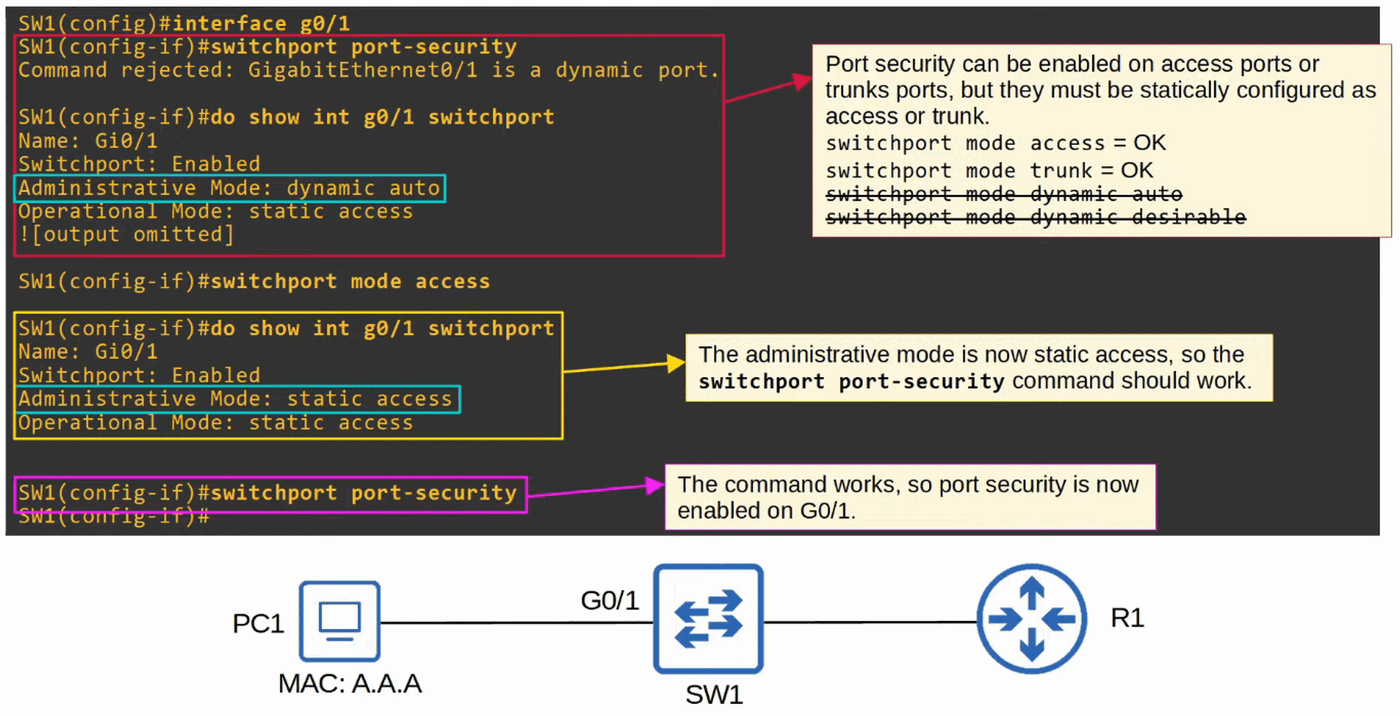
\includegraphics[keepaspectratio,alt={image}]{images/50-port-security/img-003.png}}
\end{figure}

\passthrough{\lstinline!show port-security interface!}

\begin{figure}
\centering
\pandocbounded{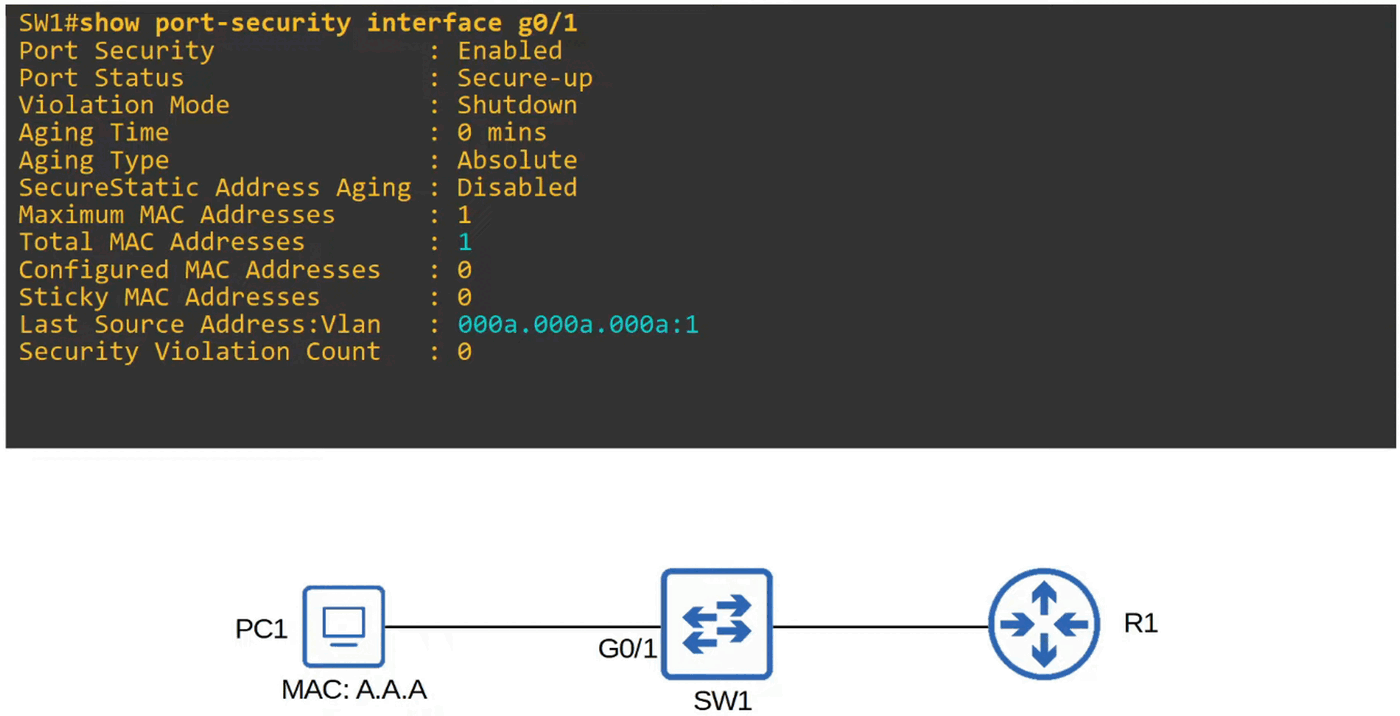
\includegraphics[keepaspectratio,alt={image}]{images/50-port-security/img-004.png}}
\end{figure}

\begin{figure}
\centering
\pandocbounded{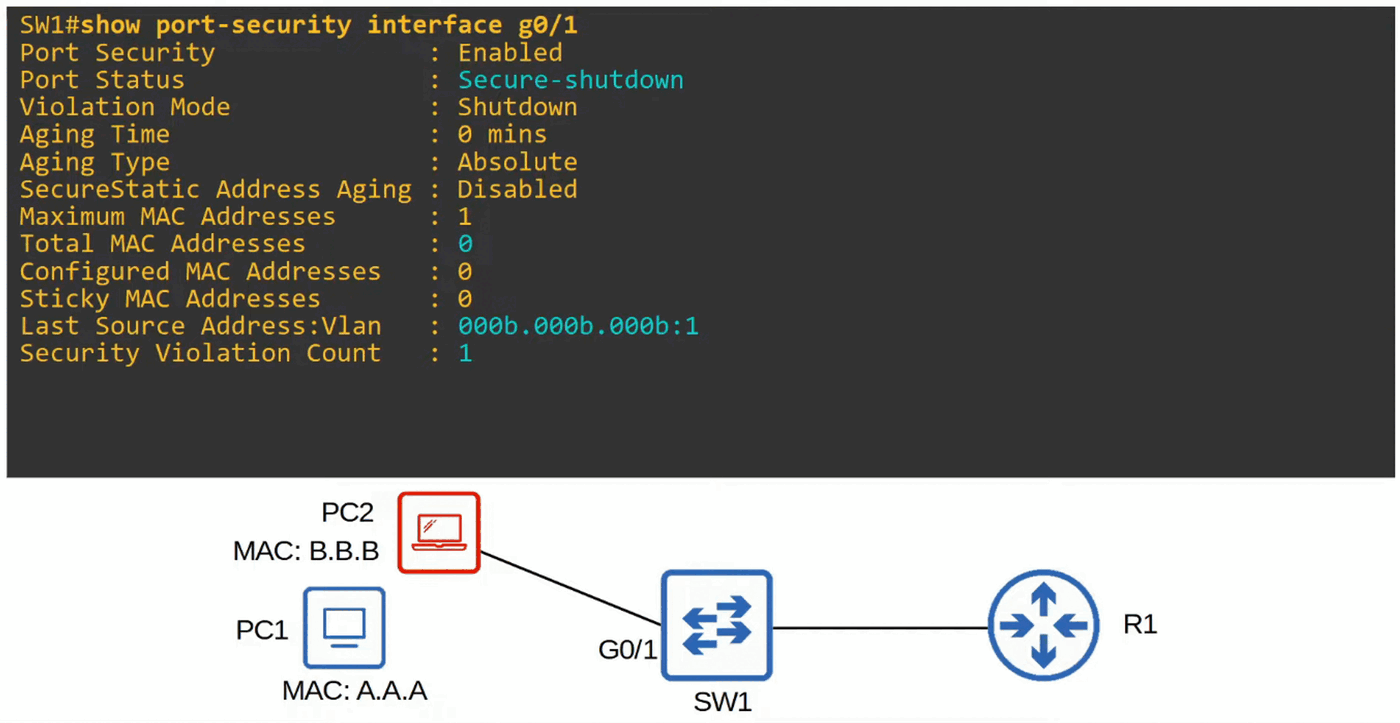
\includegraphics[keepaspectratio,alt={image}]{images/50-port-security/img-005.png}}
\end{figure}

\begin{figure}
\centering
\pandocbounded{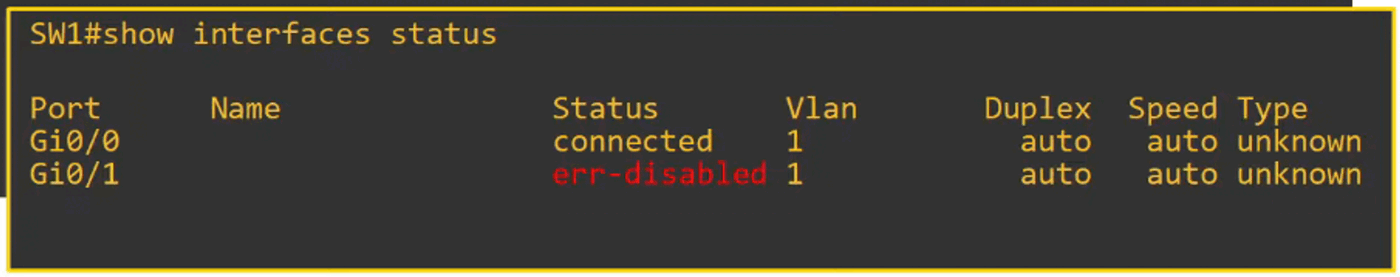
\includegraphics[keepaspectratio,alt={image}]{images/50-port-security/img-006.png}}
\end{figure}

\section{Re-Enabling an Interface
(Manually)}\label{re-enabling-an-interface-manually}

\begin{figure}
\centering
\pandocbounded{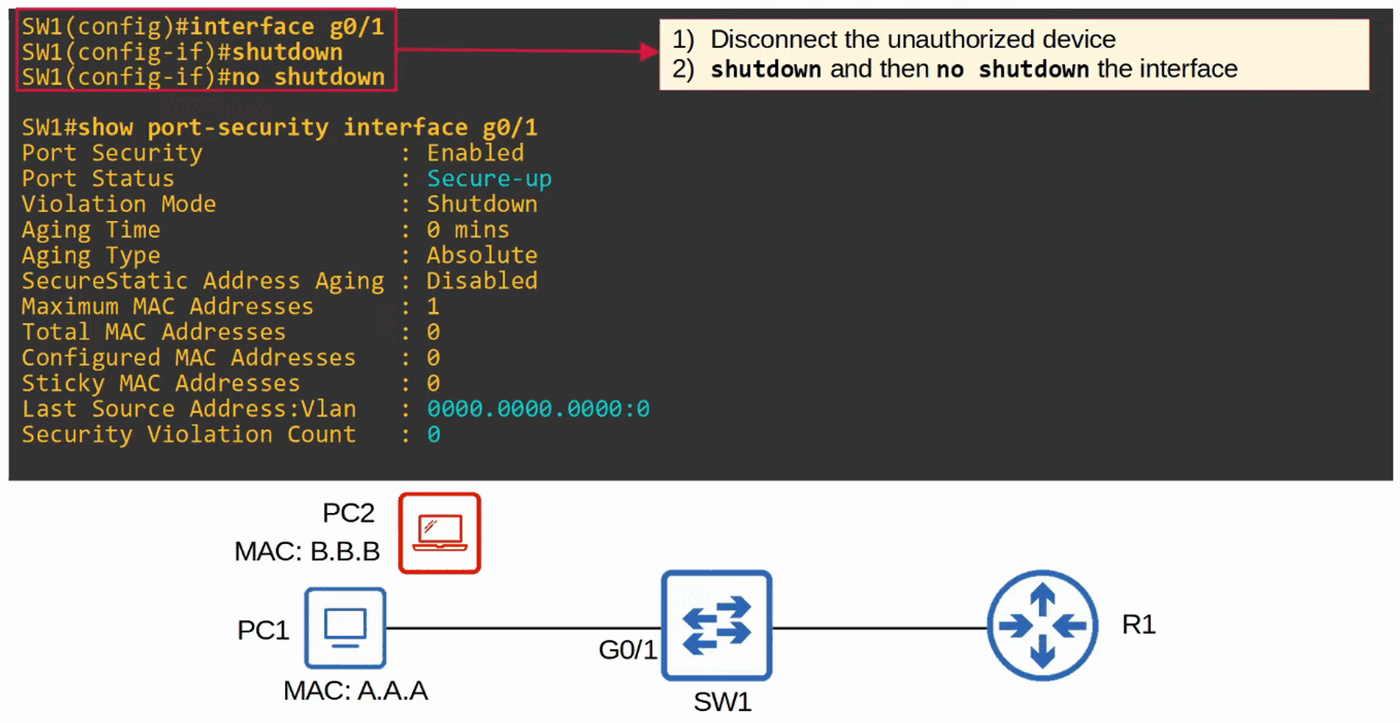
\includegraphics[keepaspectratio,alt={image}]{images/50-port-security/img-007.png}}
\end{figure}

\section{Re-Enabling an Interface (Err-Disable
Recovery)}\label{re-enabling-an-interface-err-disable-recovery}

\begin{figure}
\centering
\pandocbounded{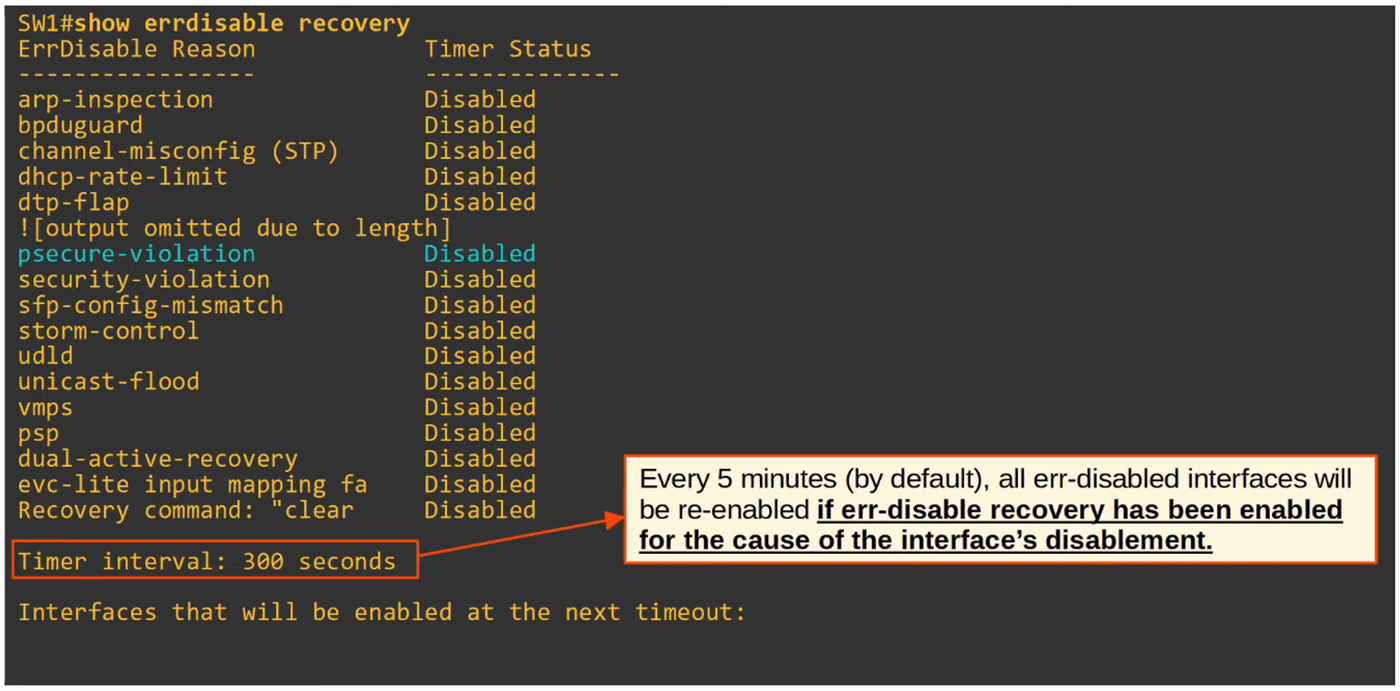
\includegraphics[keepaspectratio,alt={image}]{images/50-port-security/img-008.png}}
\end{figure}

\begin{figure}
\centering
\pandocbounded{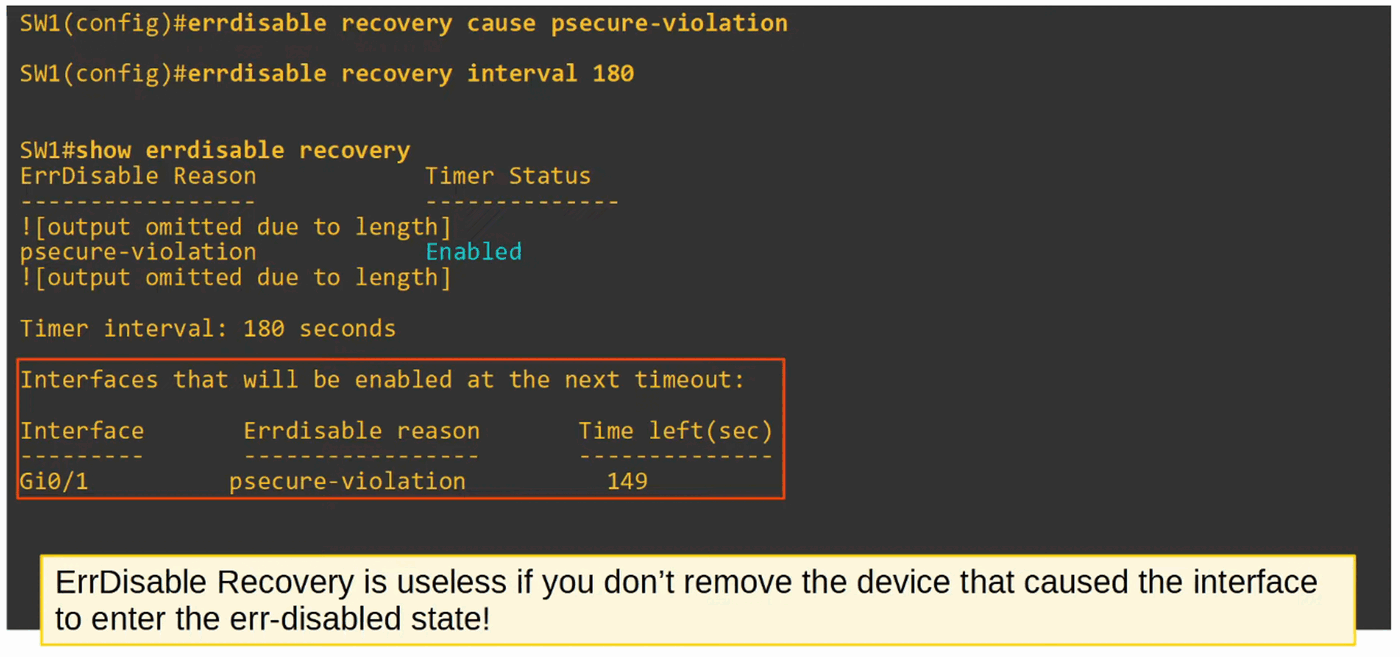
\includegraphics[keepaspectratio,alt={image}]{images/50-port-security/img-009.png}}
\end{figure}

\section{Violation Modes}\label{violation-modes}

\begin{itemize}
\tightlist
\item
  There are THREE DIFFERENT VIOLATION MODES that determine what the
  SWITCH will do if an unauthorized FRAME enters an INTERFACE configured
  with PORT SECURITY

  \begin{itemize}
  \tightlist
  \item
    SHUTDOWN

    \begin{itemize}
    \tightlist
    \item
      Effectively shuts down the PORT by placing it in an `err-disabled`
      state
    \item
      Generates a SYSLOG and / or SNMP message when the INTERFACE is
      `disabled'
    \item
      The VIOLATION counter is set to 1 when the INTERFACE is `disabled'
    \end{itemize}
  \item
    RESTRICT

    \begin{itemize}
    \tightlist
    \item
      The SWITCH discards traffic from unauthorized MAC ADDRESSES
    \item
      The INTERFACE is NOT disabled
    \item
      Generates a SYSLOG and / or SNMP message each time an unauthorized
      MAC is detected
    \item
      The VIOLATION counter is incremented by 1 for each unauthorized
      FRAME
    \end{itemize}
  \item
    PROTECT

    \begin{itemize}
    \tightlist
    \item
      The SWITCH discards traffic from unauthorized MAC ADDRESSES
    \item
      The INTERFACE is NOT disabled
    \item
      It does NOT generate a SYSLOG / SNMP message for unauthorized
      traffic
    \item
      It does NOT increment the VIOLATION counter
    \end{itemize}
  \end{itemize}
\end{itemize}

\section{Violation Mode - Restrict}\label{violation-mode---restrict}

\begin{figure}
\centering
\pandocbounded{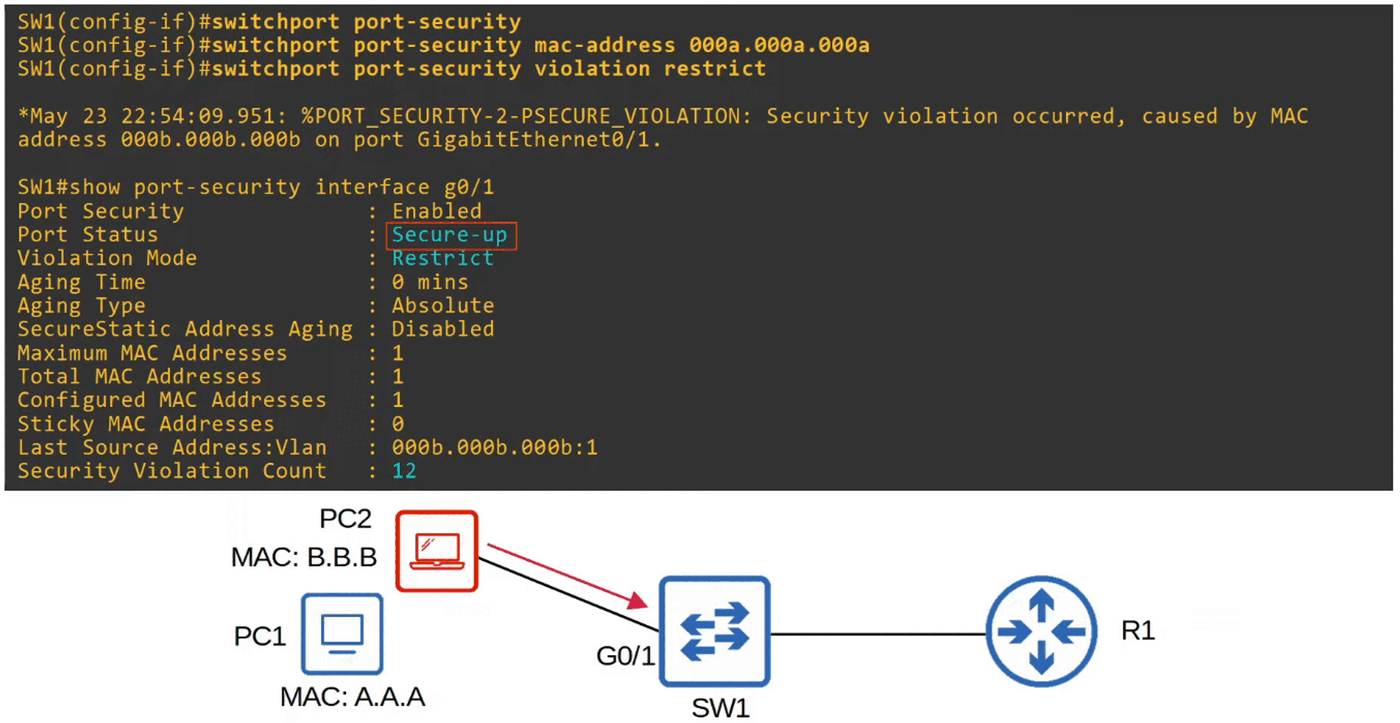
\includegraphics[keepaspectratio,alt={image}]{images/50-port-security/img-010.png}}
\end{figure}

\section{Violation Mode - Protect}\label{violation-mode---protect}

\begin{figure}
\centering
\pandocbounded{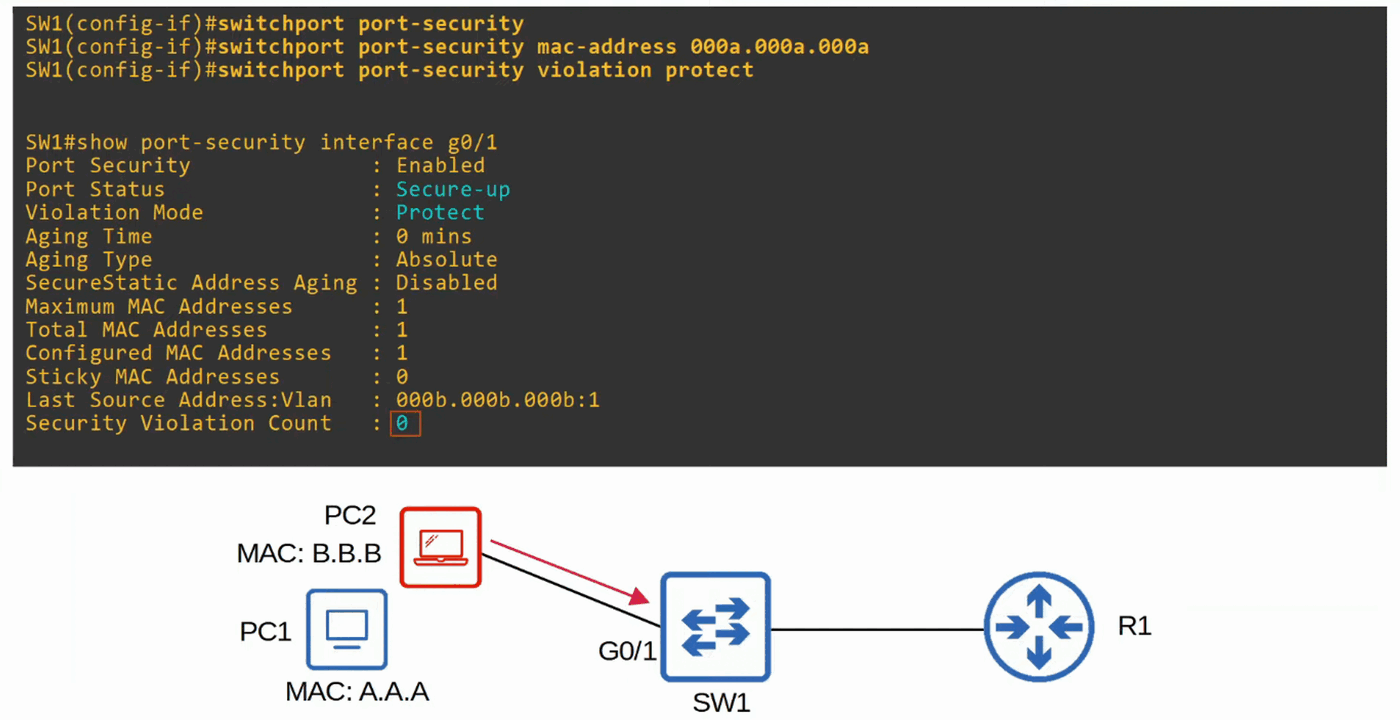
\includegraphics[keepaspectratio,alt={image}]{images/50-port-security/img-011.png}}
\end{figure}

\section{Secure MAC Address Aging}\label{secure-mac-address-aging}

\begin{figure}
\centering
\pandocbounded{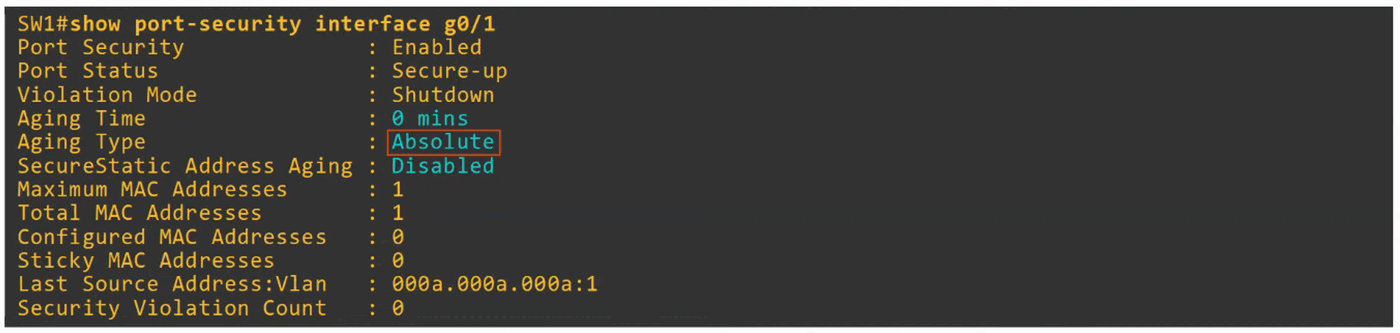
\includegraphics[keepaspectratio,alt={image}]{images/50-port-security/img-012.png}}
\end{figure}

\begin{itemize}
\tightlist
\item
  By DEFAULT, SECURE MAC ADDRESSES will not `age out' (Aging Time : 0
  mins)

  \begin{itemize}
  \tightlist
  \item
    Can be configured with
    \passthrough{\lstinline!switchport port-security aging time *minutes*!}
  \end{itemize}
\item
  The DEFAULT Aging Type is ABSOLUTE

  \begin{itemize}
  \tightlist
  \item
    ABSOLUTE

    \begin{itemize}
    \tightlist
    \item
      After the SECURE MAC ADDRESS is learned, the AGING TIMER starts
      and the MAC is removed after the TIMER expires, even if the SWITCH
      continues receiving FRAMES from that SOURCE MAC ADDRESS.
    \end{itemize}
  \item
    INACTIVITY

    \begin{itemize}
    \tightlist
    \item
      After the SECURE MAC ADDRESS is learned, the AGING TIMER starts
      but is RESET every time a FRAME from that SOURCE MAC ADDRESS is
      received on the INTERFACE

      \begin{itemize}
      \tightlist
      \item
        Aging type is configured with:
        \passthrough{\lstinline!switchport port-security aging type \{absolute | inactivity\}!}
      \end{itemize}
    \end{itemize}
  \end{itemize}
\item
  Secure Static MAC AGING (address configured with
  \passthrough{\lstinline!switchport port-security mac-address x.x.x!})
  is DISABLED by DEFAULT
\end{itemize}

\begin{figure}
\centering
\pandocbounded{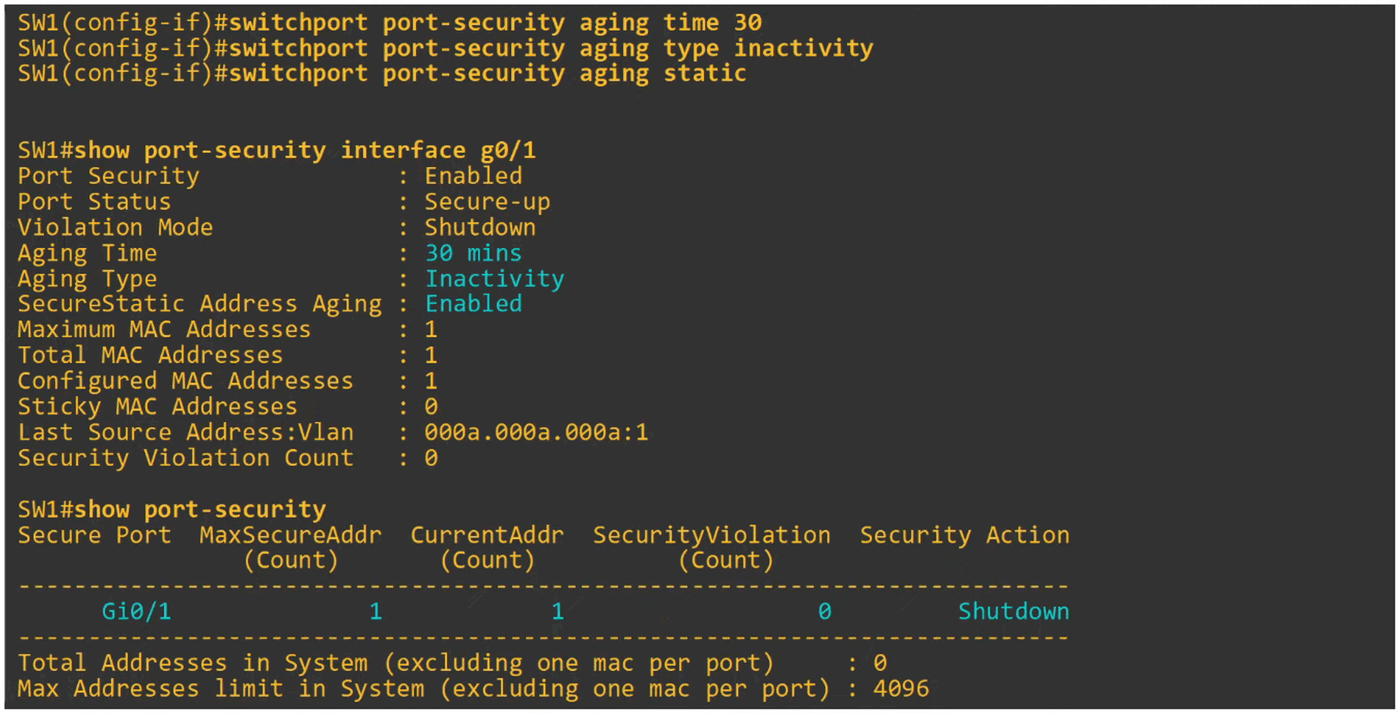
\includegraphics[keepaspectratio,alt={image}]{images/50-port-security/img-013.png}}
\end{figure}

\section{Sticky Secure MAC Addresses}\label{sticky-secure-mac-addresses}

\begin{itemize}
\tightlist
\item
  `STICKY' SECURE MAC ADDRESS learning can be enabled with the following
  command:

  \begin{itemize}
  \tightlist
  \item
    \passthrough{\lstinline!SW(config-if)\# switchport port-security mac-address sticky!}
  \end{itemize}
\item
  When enabled, dynamically-learned SECURE MAC ADDRESSES will be added
  to the running configuration, like this:

  \begin{itemize}
  \tightlist
  \item
    \passthrough{\lstinline!switchport port-security mac-address sticky *mac-address*!}
  \end{itemize}
\item
  The `STICKY' SECURE MAC ADDRESSES will NEVER age out

  \begin{itemize}
  \tightlist
  \item
    You need to SAVE the \passthrough{\lstinline!running-config!} to
    \passthrough{\lstinline!startup-config!} to make them TRULY
    permanent (or else they will not be kept if the SWITCH restarts)
  \end{itemize}
\item
  When you issue the
  \passthrough{\lstinline!switchport port-security mac-address sticky!}
  command, all current dynamically-learned secure MAC addresses will be
  converted to STICKY SECURE MAC ADDRESSES
\item
  If you issue the
  \passthrough{\lstinline!no switchport port-security mac-address sticky!}
  command, all current STICKY SECURE MAC ADDRESSES will be converted to
  regular dynamically-learned SECURE MAC ADDRESSES
\end{itemize}

\begin{figure}
\centering
\pandocbounded{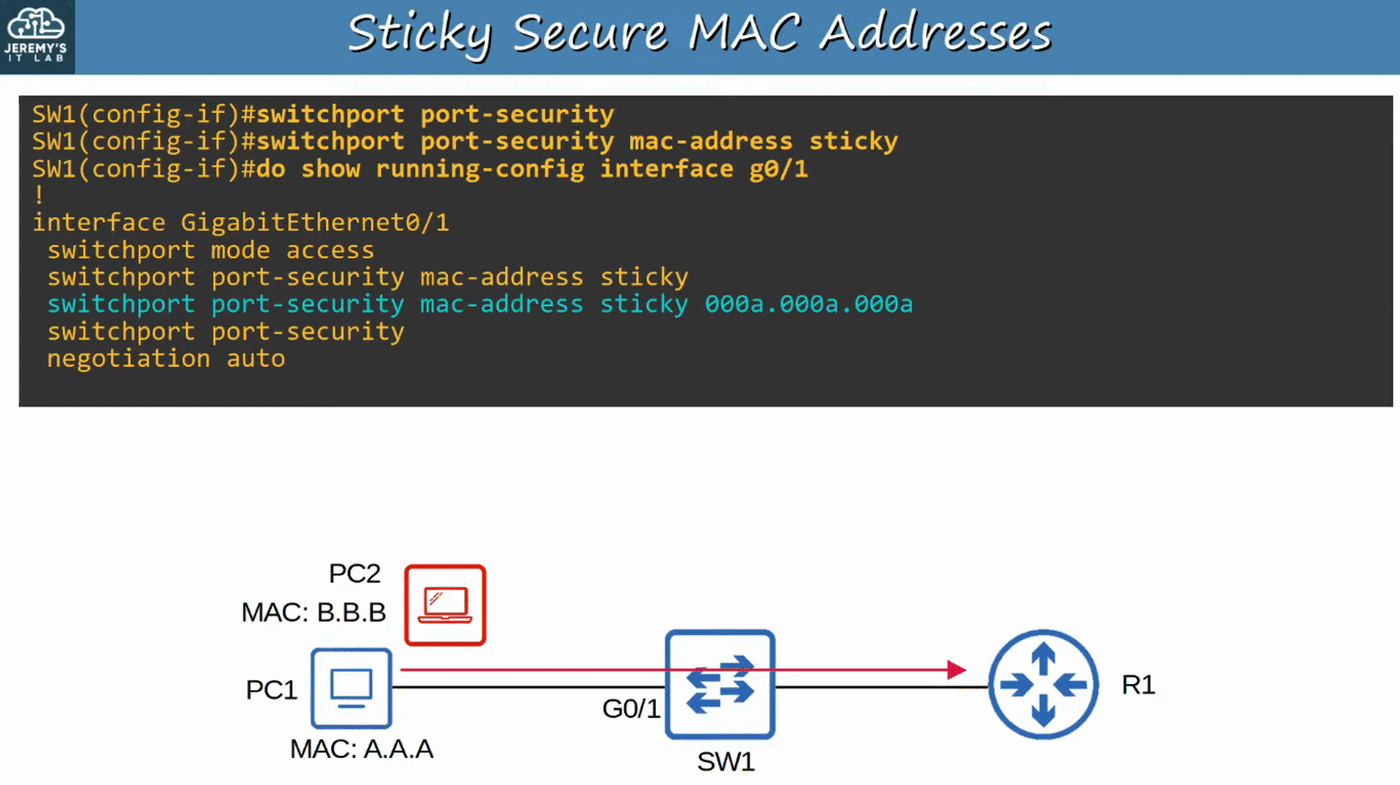
\includegraphics[keepaspectratio,alt={image}]{images/50-port-security/img-014.png}}
\end{figure}

\section{MAC Address Table}\label{mac-address-table}

\begin{itemize}
\tightlist
\item
  SECURE MAC ADDRESSES will be added to the MAC ADDRESS TABLE like any
  other MAC ADDRESS

  \begin{itemize}
  \tightlist
  \item
    STICKY and STATIC SECURE MAC ADDRESSES will have a type of STATIC
  \item
    Dynamically-Learned SECURE MAC ADDRESSES will have a type of DYNAMIC
  \item
    You can view all SECURE MAC ADDRESSES with
    \passthrough{\lstinline!show mac address-table secure!}
  \end{itemize}
\end{itemize}

\begin{figure}
\centering
\pandocbounded{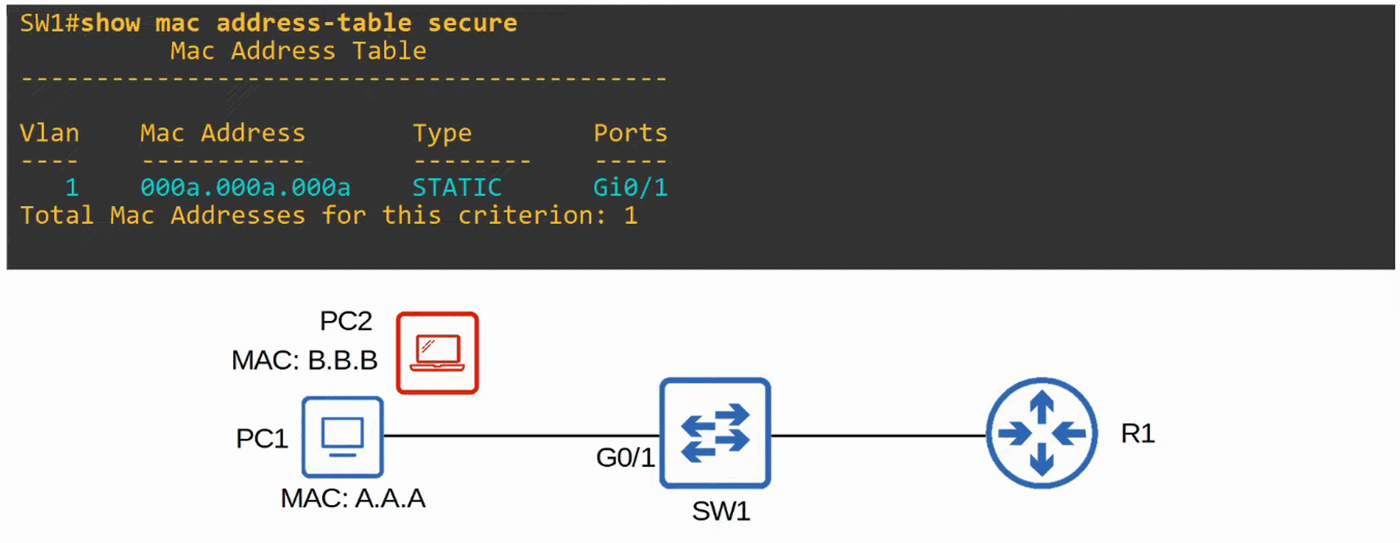
\includegraphics[keepaspectratio,alt={image}]{images/50-port-security/img-015.png}}
\end{figure}

\section{Command Review}\label{command-review}

\begin{figure}
\centering
\pandocbounded{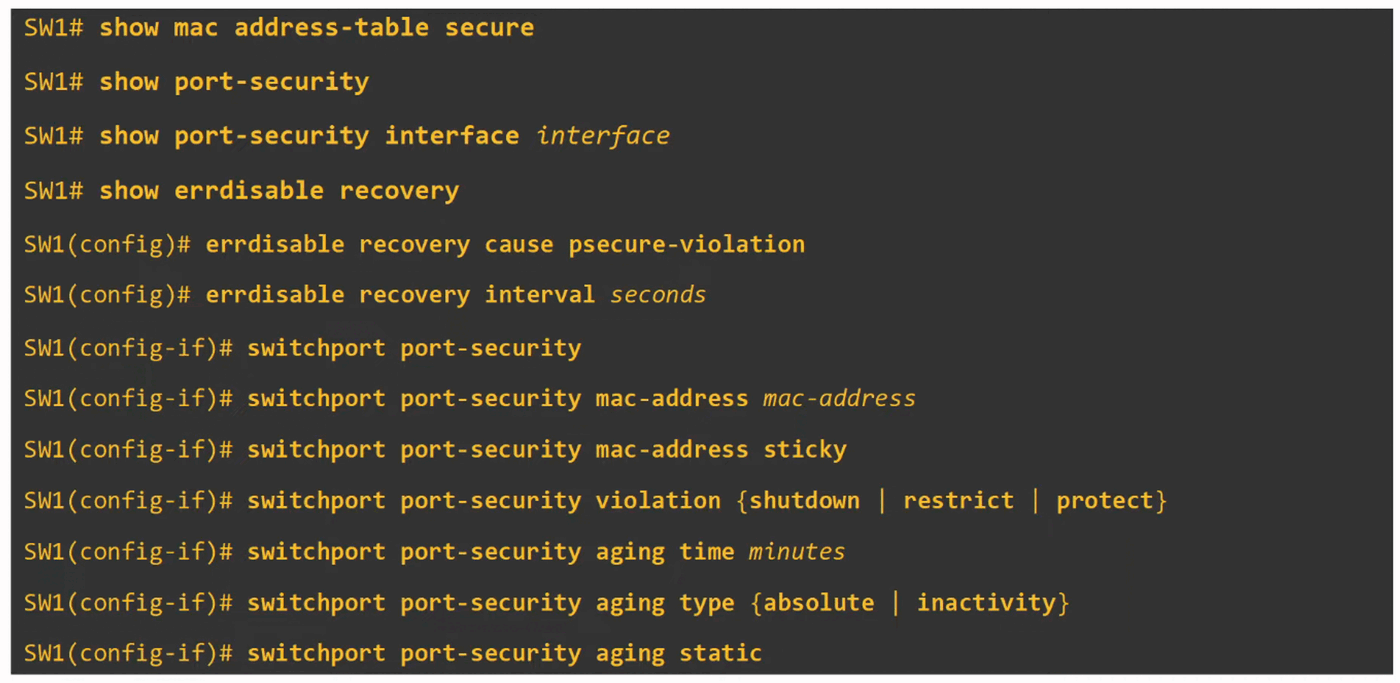
\includegraphics[keepaspectratio,alt={image}]{images/50-port-security/img-016.png}}
\end{figure}
